\section{Experimental evaluation}
\label{section:experiments}

In this section, we present some rudimentary experimental evaluation of the 
IPTV streaming service. Basically, we will present the results for the 
following key performance indicators: (i) time required to execute separate 
blocks of code, such as stream encryption, stream processing, etc; (ii) 
overall CPU load as a function of time (on both client and server); (iii) 
memory usage as a function of time (on the server only); and finally, (iv) utilized network 
bandwidth.

The first experiment we have conducted was microbanchmarking of AES encryption
on Raspberry PI. For each file of size $2^i$ megabytes, where $i \in [0, 7]$,
we have performed $100$ rounds of encryption and derived mean encryption time. We 
report the running times in seconds in Figure~\ref{fig:aes_enc}. Basically,
the running time is negligible for small streams and grows linearly with the size of 
the plaintext. In our prototype, the size of the segment was set to just $4$MB. The mean 
encryption time for such segment size is about $600$ms, which constitutes about $5-6\%$
from segment duration, and thus should not cause delays.

\begin{figure}[!h]
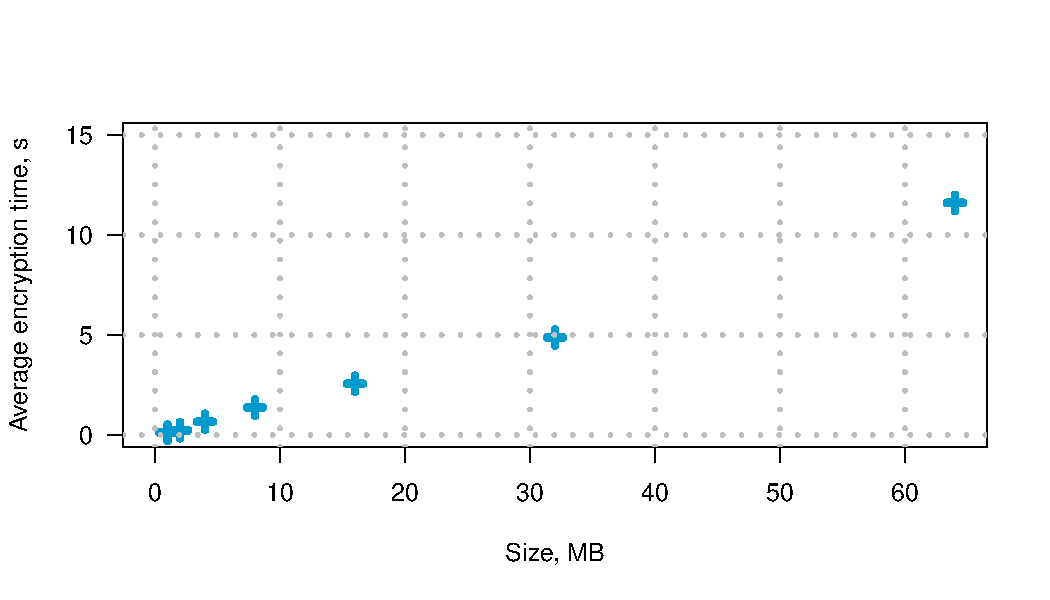
\includegraphics[width=0.5\textwidth]{graphics/microbanchmarking/aes_encryption_duration.pdf}
\caption{Microbanchmarking of AES encryption operation}
\label{fig:aes_enc}
\end{figure}

Our next experiment was related to re-encoding the audio signal. It turned out that
\textit{Flash} player - a common add-on to browsers, which is used for playing videos - does 
not support audio signal, encoded with MPEG2 audio codec. Since our content 
provider was broadcasting audio encoded with this codec, we required to transcode 
each segment using \texttt{AAC} audio codec. It was in our interest, thus, to 
benchmark the performance of this operation. In Figure~\ref{fig:aac_enc} we plot 
the mean time for this operation as a function of time, during which the signal 
was recorded. Again the mean time to re-encode the segment of size $4$MB was about
$1500$ms, or $13-15\%$ from the segment duration. Together with encryption, both operations
require just $2.1$ seconds, and should not cause any delays in video playback on the 
client - our experience with working prototype confirmed this. 

\begin{figure}[!h]
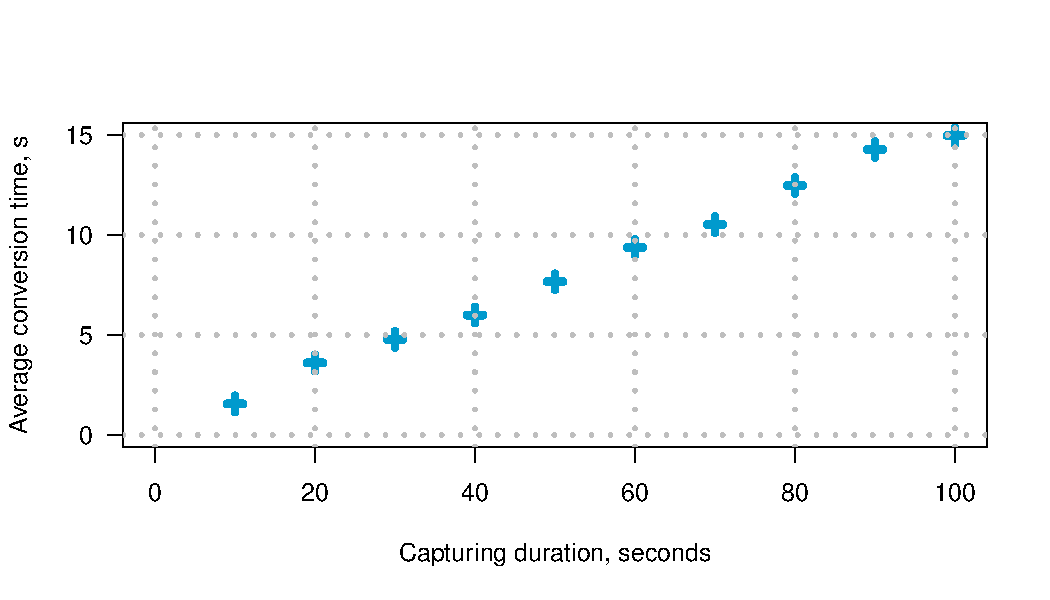
\includegraphics[width=0.5\textwidth]{graphics/microbanchmarking/mpeg2_ts_conversion.pdf}
\caption{Microbanchmarking of audio transcoding operation}
\label{fig:aac_enc}
\end{figure}

In Figure~\ref{fig:running} we demonstrate the running prototype (we tested
stream decoding in both browser (using Flash player) and 
\textit{ffplay} - desktop application). The server
was configured to encrypt the segments with the AES-128 algorithm in CBC
mode and was also transcoding the audio stream from MPEG-2 audio into 
AAC audio format. In order to understand the burden of capturing, 
re-encoding and encryption processes, we set down and measured the 
CPU utilization. For that matter, in Figure~\ref{fig:cpu_server} we show histogram 
and timeseries plot for the typical CPU utilization. From the data, 
we derived the mean CPU utilization, which was somewhere around $11\%$ 
(whereas maximum value was reaching $55\%$).
Basically, this  means that the board is capable of processing several 
MPEG-TS streams without a problem. 
In this pace, we have also measured the CPU utilization, when audio and video streams 
for four channels were captured using a single board. In Figure~\ref{fig:cpu_server_four_channles}
we show the histogram for this data. From the data, we derived
the mean CPU utilization, which was slightly more than $48\%$. 
%However, we have noticed that delays can (sometimes) occur in the playback.
To exclude IO bottleneck we have mounted \texttt{RAM} file system, 
and the capturing process was saving MPEG-TS streams to this file system.
We have noticed that the best quality and viewing experience was achieved for
the setup with one channel per computing and capturing device.

To support more channels, a production setup should have at least one processing 
and signal demodulation devices per two channels. To serve the video a load balancer
(an HTTP router) should be placed in front servers. The main role of the load balancer is 
to route HTTP requests to proper server based on the client's IP address.

\begin{figure}[ht]
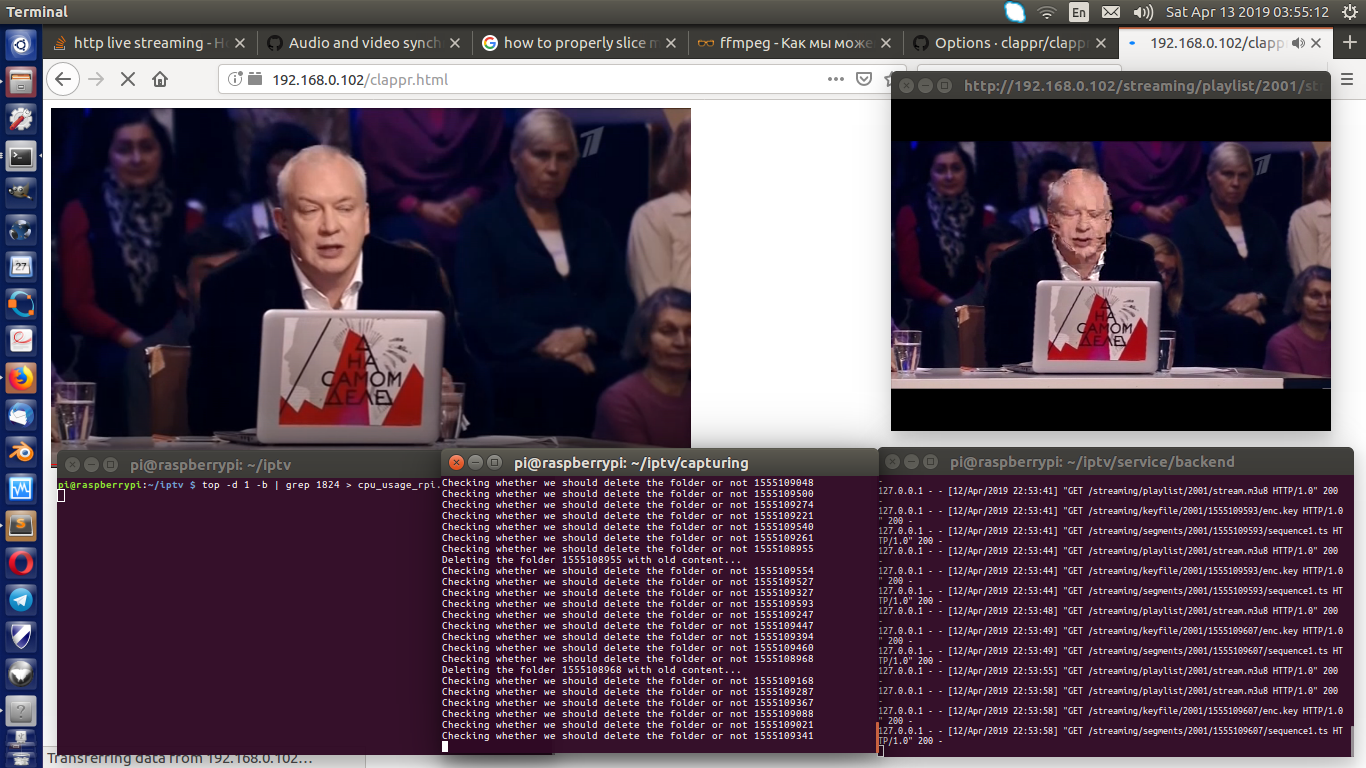
\includegraphics[width=0.5\textwidth]{graphics/running.png}
\caption{Running prototype}
\label{fig:running}
\end{figure}

We have also measured the CPU utilization on the client.
In Figure~\ref{fig:cpu_client} we show histogram and timeseries
plot for this data. Here, the mean CPU utilization was roughly $44\%$, whereas 
maximum value was reaching $93\%$.

\begin{figure}[ht]
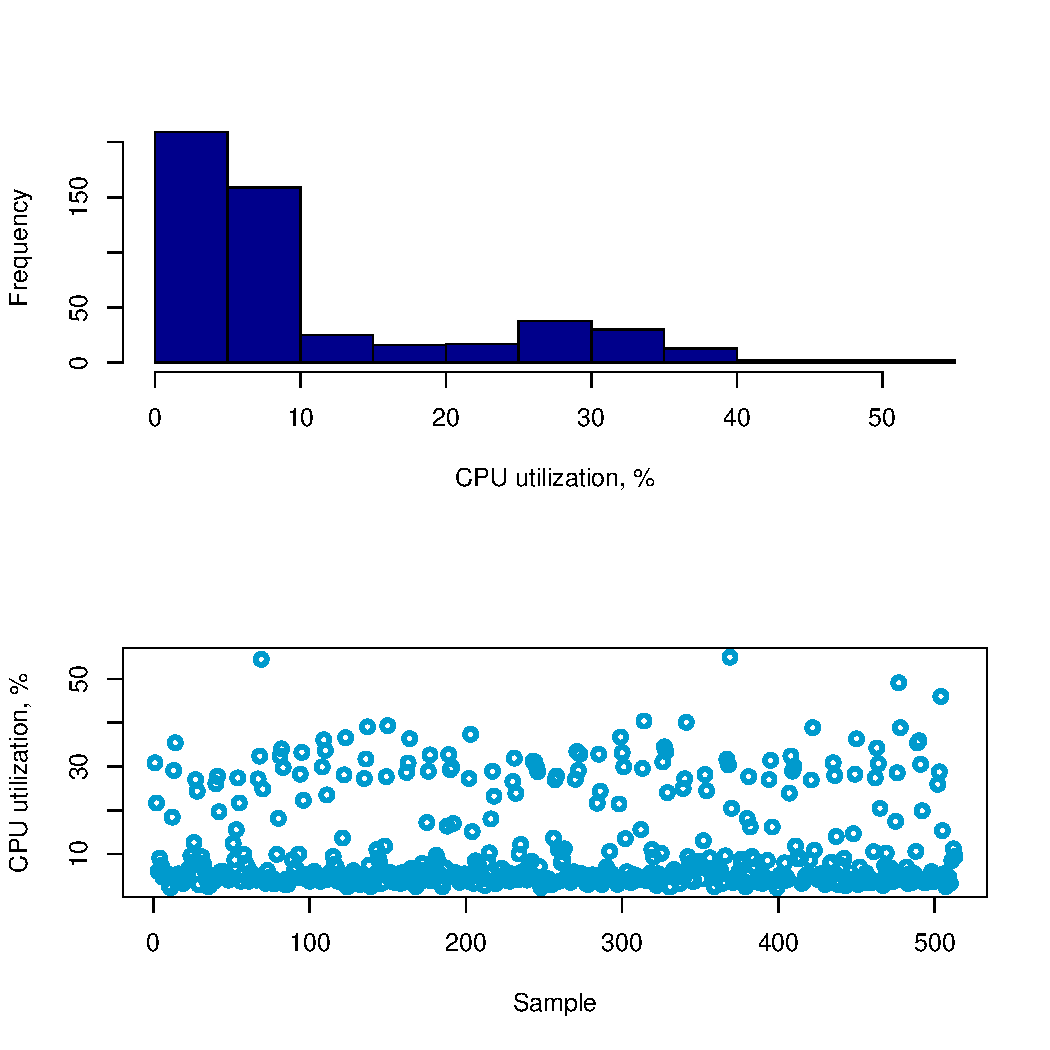
\includegraphics[width=0.5\textwidth]{graphics/microbanchmarking/cpu_usage_rpi.pdf}
\caption{CPU utilization on the server (single channel)}
\label{fig:cpu_server}
\end{figure}

\begin{figure}[ht]
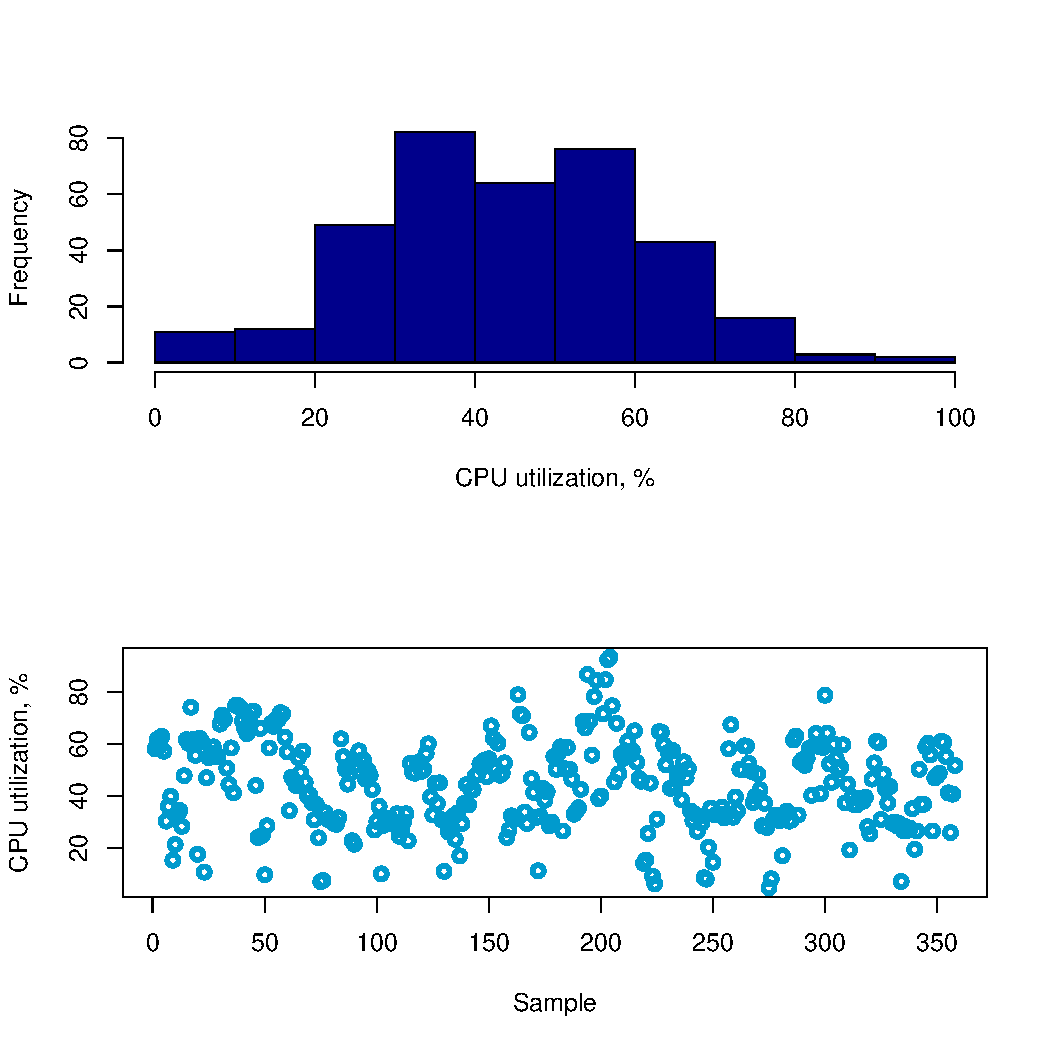
\includegraphics[width=0.5\textwidth]{graphics/microbanchmarking/cpu_usage_client.pdf}
\caption{CPU utilization on client (only for Flash player)}
\label{fig:cpu_client}
\end{figure}

\begin{figure}[ht]
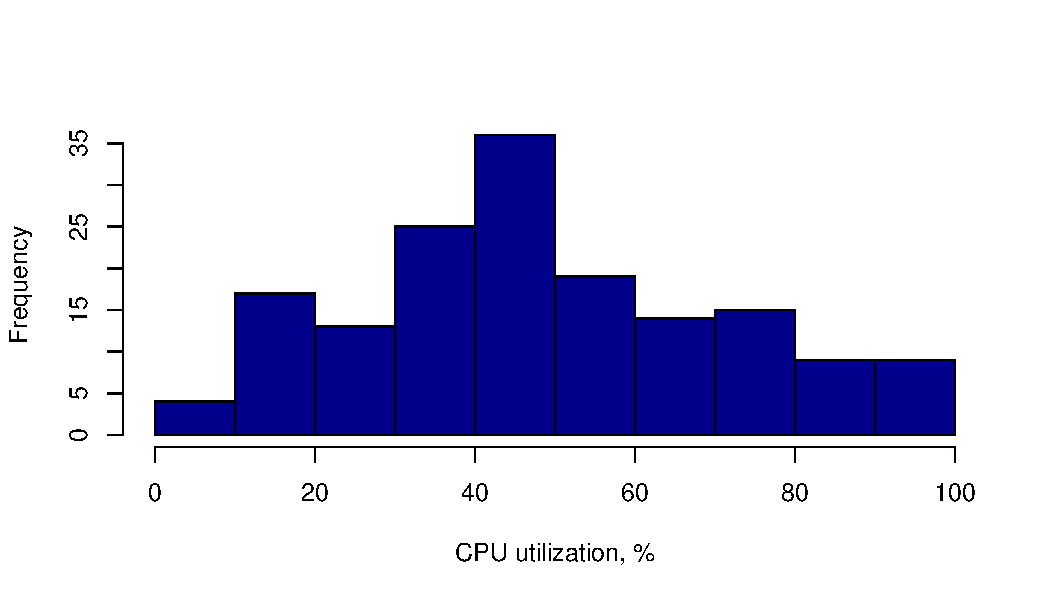
\includegraphics[width=0.5\textwidth]{graphics/microbanchmarking/cpu_usage_rpi_4_channels.pdf}
\caption{CPU utilization on server (demultiplexing four channels)}
\label{fig:cpu_server_four_channles}
\end{figure}

Our next step was to measure the average network utilization. It turned out,
that roughly $3.2$ Mb/s channel was needed to serve a single client. Back of 
the envelope calculation suggests that a $1$ gigabit link can provide enough 
capacity for $300$ concurrent clients. To improve the performance (increase the number 
of concurrent users) a multicast protocol (or IGMP) should be used. In this case, 
of course, to our best knowledge HLS protocol is not usable, and Real-time 
Transport Protocol (RTP) should be considered instead. This configuration is outside 
of the scope of this paper, but on a high level, in this setup the server simply sends 
RTP packets (which contain MPEG-TS data) to a multicast IP address and the clients, 
which are subscribed to the group will receive and decode the MPEG-TS payloads. 
A further discussion on how to encapsulate MPEG-TS stream into RTP packets can 
be found in~\cite{rfc2250}.


